\documentclass[11pt, a4paper]{article}
% \documentclass[11pt, a4paper]{scrartcl}

\usepackage[a4paper,lmargin={3cm},rmargin={3.5cm}, tmargin={2.5cm},bmargin = {2.5cm}]{geometry}
\usepackage{setspace}
\usepackage{indentfirst}
\onehalfspacing
\usepackage{enumitem}
\usepackage{amsmath, amssymb}
\usepackage{graphicx}

\newcommand{\mh}[1]{\noindent\emph{#1}}
\newcommand{\Ssa}{S_{\sigma\alpha}}
\newcommand{\Stsa}{S^t_{\sigma\alpha}}
\newcommand{\sa}{{\sigma\alpha}}
\newcommand{\given}[1][]{\:#1\vert\:}
\newcommand{\Sm}{\Stsa m^t_{\sa}}
\renewcommand{\i}[1]{\emph{#1}}
\renewcommand{\a}{\alpha}

\usepackage[backend=biber, authordate, ibidtracker=context]{biblatex-chicago}
\addbibresource{preemption.bib}

\title{\textbf{How to Deal With Expert Testimony?} \\Preemption View and Total Evidence View tested in the Olsson and Vallinder Model for Social Networks }
\author{Class Paper: Formal Methods II \\ MCMP @ LMU Munich \\ Conrad Friedrich \\ \texttt{conradfriedrich@posteo.net}}

\begin{document}

\maketitle
\abstract{}
\section{Introduction}
How to deal with expert testimony? Mention Goldman, Elga etc.

Show position by Kelly
Show position of Constantin and Grundmann

Show need to make this precise. In the case of preemption view, how to model? 
kelly's TEV for credences is just the same as bayesianism 

How to evaluate the rational strategy formally?
Epistemic Value!

\section{Model Description}

The Model used in this paper follows the one proposed by \textcite{Olsson2013} rather closely. I adopt most of their formalizations and assumptions. To enable the reader to make use of the derivations in \textcite{Angere2010}, I adopt their notations as well. I summarize the model, describe how I use it for the present purposes and make note of any deviation.

The core entities of the model are \i{agents} and their properties. Agents can be connected to one another, such that they form a network. Since these connections enable communication and the agents are meant to represent people, this structure can be seen as a social network.

The model has certain starting parameters, which I describe below, and discrete timesteps. Each of these enable the update of properties by the rules specified further below.

\subsection{Starting Parameters}

To keep things manageable, there is a single \i{true} target propostion $p$ which the agents have a credence $C^t_\alpha(p)$ towards. Each timestep, agents can receive information from a \i{source}. These can be (i) other agents in the social network or (ii) their own inquiry. The objective chance that an agents inquires and gets it right is called that agent $\alpha$'s \i{aptitude}: $P(S_{\iota \alpha}p \given S_{\iota \alpha} \land p)$, where $S_{\iota \alpha}$ is the chance that agent $\alpha$ inquires for evidence, regardless of the results, and $S_{\iota \alpha} p$ the chance that she inquires and her inquiry yields $p$ as a result. The chance that she inquires at all, $P(S_{\iota \alpha})$, is called her \i{activity}. For the sake of simplicity, these chances are modeled as time invariant.

Sources can be more or less reliable. The reliability is assumed to be symmetric.
\[ 
R_{\sigma \alpha} =_{df.} P(\Ssa p \given \Ssa \land p) = P(\Ssa \neg p \given \Ssa \land \neg p)
\]
This is, of course, just the agent's aptitude. 

Each agent trusts each source to a certain extent. This is expressed in the agent's credence in the reliability of the source:
\[ 
    C^t_{\alpha}(a \leqslant R_{\sa} \leqslant b) = \int_a^b \tau^t_{\sa}(\rho) d\rho
\]
where $\tau^t_{\sa}: [0,1] \rightarrow \mathbb{R}^+$ is a probability density function such that 
\[
    C^t_{\alpha}(0 \leqslant R_{\sa} \leqslant 1) =  \int_0^1 \tau^t_{\sa} (\rho) d(\rho) = 1
\]which is a very plausible requirement on a rational credence function.\footnote{Add Stuff here about the Olsson and Vallinder Model and how their's is slightly different.}

\begin{description}
    \item[Example.] An agent $\alpha$ with a healthy trust in her own inquisitive abilities and who is not easily swayed in this trust may have a trust function $\tau^t_{\iota\alpha}$ described by a beta distribution
\[
    \tau^t_{\iota\alpha} (\rho) = \frac{1}{B(a,b)} \rho^{a - 1} {(1 - \rho)}^{b-1}
\]
with normalising beta function $B(a,b)$ and parameters $a, b$ chosen such that $\tau^t_{\iota\alpha}$ is densest around whatever a `healthy trust' amounts to, let's say 0.85. (see Fig.\ref{fig1}). Interestingly, the shape of the curve correlates with how resilient the funtion behaves upon updating. More on that below.
\end{description}

\begin{figure}[ht]
	\centering\label{fig1}
    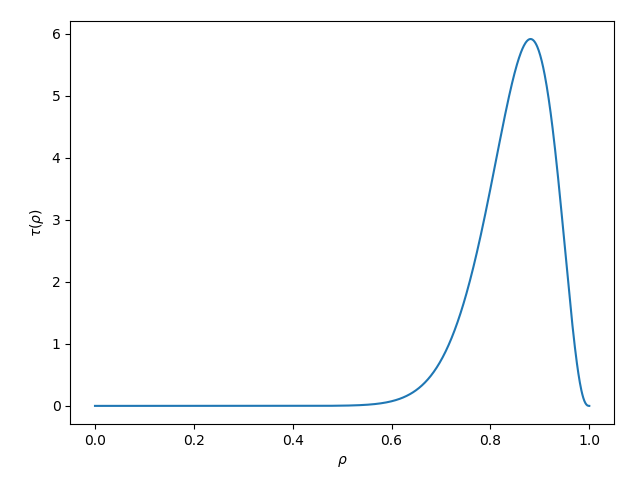
\includegraphics[width=0.5\textwidth]{Figure_1.png}
	\caption{Example beta distributed trust function with parameters a=LOOK b=UP }
\end{figure}

Apart from inquiries, a source can also be another agent, through testimony. An agent $\alpha$ therefore trusts herself at time $t$ with $\tau^t_{\iota\alpha}$ and another agent $\beta$ with $\tau^t_{\beta\alpha}$.

The exchange of information and the evolution of the trust functions and the credences in $p$ are the most important going-ons in this model, which I'll summarize next.

\subsection{Inquiry and Communication} 

time progess is modeled in discrete steps. At each time step, each agent updates her credence and her trust function. The new information which motivates these changes are messages from the sources, which the agent receives if
\begin{enumerate}[label = (\roman*)]
    \item the agent inquires herself with probability $P(S_{\iota\alpha})$. The result of the inquiry is determined by the agent's aptitude. Or,
    \item another agent $\beta$ is connected to agent $\alpha$ through the social network and decides to share her opinion. This is modeled, in slight deviation from the Olsson-Vallinder model, by the following conditions: 
        \begin{enumerate}[label = (\alph*)]
            \item Agent $\beta$ is sufficiently confident in $p$ resp. $\neg p$, determined by some faily high threshold value for her credence, and
            \item agent $\beta$ received herself new information in the same time step. In the current implementation, this is only fulfilled by own inquiry.  
        \end{enumerate}
\end{enumerate}

EXPLAIN why only when new information!!

Testimony is, of course, a matter of language, and is most plausibly modeled as a binary judgment, that is, either $p$ or $\neg p$. While there are certainly interesting cases where the testimony involves credences or levels of confidences, e.g. \ a weather forecaster stating her belief in the chance of rain tomorrow, this does in my view not apply to  

\subsection{Updating}

Each time step, the agents update their credences and trust functions. Updating the credences is based on new messages the agent received this time step: $\Stsa m^t_{\sa}$, where $m^t_{\sa}$ is the message that $\alpha$ received from $\sigma$ (which can represent $\alpha$'s own inquiry or another agent's testimony) at $t$, and is either $p$ or $\neg p$. An agents can receive multiple messages per time step, but only one message per source, so we have to account for that as well: 

The updating rule is given by conditionalization:
\[
    C^{t+1}_\alpha (p) = C^t_\alpha (p \given \bigwedge_{\sigma \in \Sigma^t_\alpha} \Stsa m^t_{\sa}),
\]

where $\Sigma^t_\alpha$ is the set of sources that send a message to $\alpha$ at $t$.

With the assumption that sources are independent given the target proposition, the update calculates to
\[
    C^t_\a (p \given \bigwedge \Sm) 
    = \frac{ C^t_\a (p) \prod C^t_\a (\Sm \given p) }
    { C^t_\a (p) \prod C^t_\a (\Sm \given p) +  C^t_\a (\neg p) \prod C^t_\a (\Sm \given \neg p) }.
\]

Here, again, the product and big conjunct range over all sources with a message for the agent, now omitted for legibility.   

The expressions about the reliability are given by:

\begin{align*}
    C^t_\a (\Stsa p \given p) &= C^t_\a (\Stsa) \langle \tau^t_{\sa} \rangle \\
    C^t_\a (\Stsa \neg p \given p) &= C^t_\a (\Stsa) \langle \bar{\tau}^t_{\sa} \rangle \\
    C^t_\a (\Stsa p \given \neg p) &= C^t_\a (\Stsa) \langle \bar{\tau}^t_{\sa} \rangle \\
    C^t_\a (\Stsa \neg p \given \neg p) &= C^t_\a (\Stsa) \langle \tau^t_{\sa} \rangle,
\end{align*}

where $\langle \tau^t_{\sa} \rangle $ is the expected value of trust function $ \tau^t_{\sa} $ and ${\langle \bar{\tau}^t_{\sa} \rangle =_{df.} 1 - \langle \tau^t_{\sa} \rangle}$.\footnote{Detailed and very helpful derivations of these equations can be found in \textcite{Angere2010}, although in places I could not agree with the results. I implemented the updating mechanism as presented in this paper. There is not much room to detail the finer points here, only this much: Angere's final result on page 22 for the credence update intuitively can't be right, since the expression as stated there does not depend on the actual content of the message, that is, $p$ or $\neg p$, anymore, and instead just updates regardless, rendering the network communication ineffective.} 

Upon each message received, the agents updates her trust function for that source depending on how well the message coheres with her own credence. The updated trust function can be calculated to
\[
    \tau^{t+1}_\sa = \tau^t_\sa (\rho) \frac{\rho \: C^t_\a (p) + (1 - \rho) C^t_\a (\neg p)}
    {\langle \tau^t_\sa \rangle C^t_\a(p) + \langle \bar{\tau}^t_\sa \rangle C^t_\a(\neg p)}
\]
if $m^t_{\sa} = p$ and 
\[
    \tau^{t+1}_\sa = \tau^t_\sa (\rho) \frac{\rho \: C^t_\a (\neg p) + (1 - \rho) C^t_\a (p)}
    {\langle \tau^t_\sa \rangle C^t_\a(\neg p) + \langle \bar{\tau}^t_\sa \rangle C^t_\a(p)}
\]
if $m^t_{\sa} = \neg p$. This entails that the trust an agents brings towards a source only changes with regards to the agents credence in p and the source's message whether p. This is one of the major shortcomings of the model, in my view, especially for the current purposes, as at no stage something like higher order evidence about the reliability of the source comes into play. 

Insert example with trust function development?

\subsection{Epistemic Value}





Agent's properties
Communication. Diverges from Constantin and Grundmann
Reliability
Updating etac\
esp. \ the time step issue. \ can repeated statements of the authority really be independent of the ones before?
Epistemic Value
CENTRAL ASSUMPTIONS

\section{Experiment}
How to setup a specific experiment? Expert Layperson structure, how to set up credences, metadistributions, 

\section{Experiment: Results}

\nocite{*}
\printbibliography{}
\end{document}

